\nextchapter{State Feedback and Observer Design (\textit{LTI only})}
\begin{Theorem}
Consider system $\{A,B,C,D\}$ and change of basis $\widetilde x=Tx\forall t\in\Reals_+,T\in\Reals^{n\times n}$ invertible. Then:
\begin{enumerate}[leftmargin=4mm]
  \item In new basis $\{\widetilde A=TAT^{-1},\widetilde B=TB,\widetilde C=CT^{-1},\widetilde D=D\}$
  \item $\Spec[A]=\Spec[\widetilde A]$
  \item $\widetilde G(s)=\widetilde C(sI-A)^{-1}\widetilde B+\widetilde D=C(sI-A)^{-1}+D=G(s)$
  \item $(\widetilde A,\widetilde B)$ controllable $\Leftrightarrow$ $(A,B)$ controllable.
  \item $(\widetilde C,\widetilde A)$ observable $\Leftrightarrow$ $(C,A)$ observable.
\end{enumerate}
\end{Theorem}





\nextsubchapter{Linear state feedback for single-input (SI) systems}
\begin{Definition}
Let char. poly. $\Det[\lambda I-A]=\lambda^n+\chi_1\lambda^{n-1}+\cdots+\chi_{n-1}\lambda+\chi_n$. Define matrix $S$ w/ $\{s_n=B,s_{n-k}=As_{n-k+1}+\chi_kB\}$:
\begin{equation*}
\def\arraycolsep{1pt}
S=\begin{bmatrix}
s_1 & \cdots & s_n
\end{bmatrix}=\begin{bmatrix}
B & AB & \cdots & A^{n-1}B
\end{bmatrix}\begin{bmatrix}
\chi_{n-1} & \chi_{n-2} & \cdots & \chi_1 & 1 \\
\chi_{n-2} & \chi_{n-3} & \cdots & 1 & 0 \vspace{-1mm} \\
\vdots & \vdots & \iddots & \vdots & \vdots \\
\chi_1 & 1 & \cdots & 0 & 0 \\
1 & 0 & \cdots & 0 & 0
\end{bmatrix}
\end{equation*}
\begin{Theorem}
$As_1+\chi_nB=0$. NB: $S\in\Reals^{n\times n}$ invertible $\Leftrightarrow$ $(A,B)$ controllable.
\end{Theorem}
\end{Definition}
\begin{Theorem}
\hl{Controllable canonical form}. $(A,B)$ controllable $\Leftrightarrow\exists T_c\in\Reals^{n\times n}$ invertible, $\widetilde x(t)=T_cx(t)$, s.t. $\widetilde A=T_cAT_c^{-1}$, $\widetilde B=T_cB$ s.t.
\begin{equation*}
\def\arraycolsep{1pt}
\widetilde A=
\begin{bmatrix}
0 & 1 & 0 & \cdots & 0 \\
0 & 0 & 1 & \cdots & 0\vspace{-1mm} \\
\vdots & \vdots & \vdots & \ddots & \vdots \\
0 & 0 & 0 & \cdots & 1 \\
-\chi_n & -\chi_{n-1} & -\chi_{n-2} & \cdots & -\chi_1
\end{bmatrix},\quad\widetilde B=\begin{bmatrix}
0 \\ 0 \\ \vdots \\ 0 \\ 1
\end{bmatrix},\quad\mc{blue}{T_c^{-1}\equiv S}
\end{equation*}
\end{Theorem}
\begin{Definition}
\textbf{LTI (single-input) state feedback}: $u(t)=Kx(t)+r(t)$, $K\in\Reals^{m\times n}$ \textbf{gain matrix}, $r(t)\in\Reals$ ``ext. input vec.''. CL dynamics: $\dot x(t)=(A+BK)x(t)+Br(t)$.
\end{Definition}
\begin{Theorem}
$(A,B)$ controllable $\Leftrightarrow\forall\{\lambda_1,\ldots,\lambda_n\}\subseteq\Complex$ $\exists K\in\Reals^{m\times n}$ s.t. $\Spec[A+BK]=\{\lambda_1,\ldots,\lambda_n\}$ (the desired \textbf{CL poles}).
\end{Theorem}
\begin{Method}
\hl{Pole placement}. Find $K$ that places CL poles at $\{\lambda_1,\ldots,\lambda_n\}$.
\begin{enumerate}[label=\protect\circled{\arabic*},leftmargin=4mm]
  \item Write $\Det[\lambda I-A]=\lambda^n+\chi_1\lambda^{n-1}+\cdots+\chi_{n-1}\lambda+\chi_n$.
  \item Write $\Det[\lambda I-(A+BK)]=(\lambda-\lambda_1)\cdots(\lambda-\lambda_n)=\lambda^n+d_1\lambda^{n-1}+\cdots+d_{n-1}\lambda+d_n$.
  \item Define $\widetilde K=[\widetilde k_n\cdots\widetilde k_1]\in\Reals^{1\times n}$. Compute $\widetilde k_i=\chi_i-d_i$ $\forall i$.
  \item Obtain $K=\widetilde KT_c=\widetilde KS^{-1}$ \QED
\end{enumerate}
OR just solve \circled{2} with $K=[k_1\cdots k_n]$ as vars ($n\times n$ lin. sys.).
\end{Method}





\nextsubchapter{LTI state observers for single-output (SO) systems}
\begin{Definition}
$C\in\Reals^{1\times n},D\in\Reals^{1\times m},u\in \Reals^m$, $L\in\Reals^{n\times 1}$ \textbf{observer gain matrix}. Then:
\begin{equation*}
\textbf{Observer\textnormal{ of }}\{A,B,C,D\}:\begin{cases}
\dot{\widehat x}=A\widehat x+Bu+L(y-\widehat y) \\
\widehat y=C\widehat x+Du
\end{cases}
\end{equation*}
\end{Definition}
\begin{Definition}
$e:=x-\widehat x$ \textbf{estimation error}. Dynamics: $\dot e(t)=(A-LC)e(t)$.
\end{Definition}
\begin{Theorem}
Estimation works $\Leftrightarrow e(t)\to 0\Leftrightarrow\text{Real}[\lambda]<0$ $\forall\lambda\in\Spec[A-LC]$.
\end{Theorem}

\begin{Theorem}
\hl{Observable canonical form}. $(C,A)$ observable $\Leftrightarrow$ $\exists T_o\in\Reals^{n\times n}$ invertible, $\widetilde x(t)=T_ox(t)$, s.t. $\widetilde A=T_oAT_o^{-1}$, $\widetilde B=T_oB$ s.t.
\begin{equation*}
\widetilde A=\begin{bmatrix}
0 & 0 & \cdots & 0 & -\chi_n \\
1 & 0 & \cdots & 0 & -\chi_{n-1} \vspace{-1mm} \\
\vdots & \vdots & \ddots & \vdots & \vdots \\
0 & 0 & \cdots & 1 & -\chi_1
\end{bmatrix},\quad\widetilde C=\begin{bmatrix}
0 & \cdots & 0 & 1
\end{bmatrix}
\end{equation*}
\begin{equation*}
\def\arraycolsep{2pt}
\text{where }T_o:=\begin{bmatrix}
\chi_{n-1} & \chi_{n-2} & \cdots & \chi_1 & 1 \\
\chi_{n-2} & \chi_{n-3} & \cdots & 1 & 0 \vspace{-1mm} \\
\vdots & \vdots & \iddots & \vdots & \vdots \\
\chi_1 & 1 & \cdots & 0 & 0 \\
1 & 0 & \cdots & 0 & 0
\end{bmatrix}\begin{bmatrix}
C \\
CA \vspace{-1mm} \\
\vdots \\
CA^{n-1}
\end{bmatrix}\mc{blue}{\equiv S^T (\text{duality})}
\end{equation*}
\end{Theorem}
\begin{Method}
\hl{Observer design}. Find $L$ that places error dynamics poles at $\{\lambda_1,\ldots,\lambda_n\}$.
\begin{enumerate}[label=\protect\circled{\arabic*},leftmargin=4mm]
  \item Write $\Det[\lambda I-A]=\lambda^n+\chi_1\lambda^{n-1}+\cdots+\chi_{n-1}\lambda+\chi_n$.
  \item Write $\Det[\lambda I-(A-LC)]=(\lambda-\lambda_1)\cdots(\lambda-\lambda_n)=\lambda^n+d_1\lambda^{n-1}+\cdots+d_{n-1}\lambda+d_n$.
  \item Define $\widetilde L=[\widetilde l_n;\cdots;\widetilde l_1]\in\Reals^{n\times 1}$. Compute $\widetilde l_i\hspace{-1.5mm}\overset{\mathcal{\text{order!}}}{=}\hspace{-1mm}d_i-\chi_i\forall i$.
  \item Obtain $L=T_o^{-1}\widetilde L$. \QED
\end{enumerate}
OR just solve \circled{2} with $L=[l_1;\cdots ; l_n]$ as vars ($n\times n$ lin. sys.).
\end{Method}
\begin{Theorem}
$(C,A)$ observable $\Leftrightarrow\forall\{\lambda_1,\ldots,\lambda_n\}\subseteq\Complex$ $\exists L\in\Reals^{m\times n}$ s.t. $\Spec[A-LC]=\{\lambda_1,\ldots,\lambda_n\}$.
\end{Theorem}





\nextsubchapter{Principle of separation}
\begin{minipage}{0.3\columnwidth}
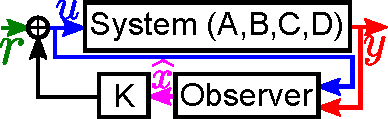
\includegraphics[height=0.33\columnwidth]{figures/separation.pdf}
\end{minipage}%
\begin{minipage}{0.7\columnwidth}
\begin{equation*}
\begin{bmatrix}
\dot x \\
\dot{\widehat x}
\end{bmatrix}=\begin{bmatrix}
A & BK \\
LC & A+BK-LC
\end{bmatrix}\begin{bmatrix}
x \\
\widehat x
\end{bmatrix}+\begin{bmatrix}
B \\
B
\end{bmatrix}r
\end{equation*}
\end{minipage}
Change basis: $[x;e]=[x;x-\widehat x]=[I,0;I,-I][x;\widehat x]=T[x;\widehat x]$.
\begin{equation*}
\Rightarrow \begin{bmatrix}
\dot x \\
\dot e
\end{bmatrix}=\begin{bmatrix}
A+BK & -BK \\
0 & A-LC
\end{bmatrix}\begin{bmatrix}
x \\ e
\end{bmatrix}+\begin{bmatrix}
B \\ 0
\end{bmatrix}r=\overline A\begin{bmatrix}
x \\ e
\end{bmatrix}+\begin{bmatrix}
B \\ 0
\end{bmatrix}r
\end{equation*}
\begin{Theorem}
$\therefore$\textbf{Princip. of separ.}: $\Spec[\overline A]=\Spec[A+BK]\union\Spec[A-LC]$

$\Rightarrow$ CL ctrlr. + obsrvr. remains stable if ctrlr. \& obsrvr. stable!
\end{Theorem}